\documentclass[format=sigplan,dvipsnames,backend=bibtex]{acmart}

%%% Top Matter %%%
\title{Extended Abstract: Flexible Structure Editing of Well-Typed Expressions}

\author{David Moon}
\affiliation{University of Colorado Boulder}
\email{dmoon1221@gmail.com}

\author{Cyrus Omar}
\affiliation{University of Chicago}
\email{cyrus.omar@gmail.com}

\author{R.~Benjamin Shapiro}
\affiliation{University of Colorado Boulder}
\email{ben.shapiro@colorado.edu}

\acmConference{TyDe’19}{August 18, 2019}{Berlin, Germany}
\acmISBN{}
\acmDOI{}

\setcopyright{none}

\settopmatter{printacmref=false}

\bibliographystyle{ACM-Reference-Format}
%\citestyle{acmauthoryear}
%%%%%%


%%% Packages + Commands %%%
\usepackage{microtype}
\usepackage{mdframed}
\usepackage{mathpartir}
\usepackage{enumitem}
\usepackage{bbm}
\usepackage{stmaryrd}
\usepackage{mathtools}
\usepackage{leftidx}
\usepackage{wrapfig}
\usepackage{extarrows}
\usepackage{xspace}
\usepackage{todonotes}
\usepackage{bm}
\usepackage{xcolor}
\usepackage{enumitem}

% https://tex.stackexchange.com/a/8633
\usepackage{float}

% inconsolata font
\usepackage{zi4}

% !TEX root = main.tex

\newcommand{\mynote}[3]{\textcolor{#3}{\textsf{{#2}}}}
\newcommand{\rkc}[1]{\mynote{rkc}{#1}{blue}}
\newcommand{\cy}[1]{\mynote{cy}{#1}{purple}}
\newcommand{\mah}[1]{\mynote{cy}{#1}{green}}
\newcommand{\matt}[1]{{\color{blue}{\textit{Matt:~#1}}}}

\newcommand{\cvert}{{\,{\vert}\,}}

%% https://tex.stackexchange.com/questions/9796/how-to-add-todo-notes
\newcommand{\rkcTodo}[1]{\todo[linecolor=blue,backgroundcolor=blue!25,bordercolor=blue]{#1}}

\newcommand{\mattTodo}[1]{\todo[linecolor=green,backgroundcolor=green!2,bordercolor=green]{\tiny\textit{#1}}}
\newcommand{\mattOmit}[1]{\colorbox{yellow}{(Matt omitted stuff here)}}

\def\parahead#1{\paragraph{\textbf{#1.}}}
%% \def\paraheadNoDot#1{\paragraph{{\textbf{#1}}}}
\def\subparahead#1{\paragraph{\textit{#1.}}}
%% \def\paraheadindent#1{\paragraph{}\textit{#1.}}
%% \def\paraheadindentnodot#1{\paragraph{}\textit{#1}}

% \newcommand{\ie}{{\emph{i.e.}}}
% \newcommand{\eg}{{\emph{e.g.}}}
% \newcommand{\etc}{{\emph{etc.}}}
% \newcommand{\cf}{{\emph{cf.}}}
% \newcommand{\etal}{{\emph{et al.}}}

%% \newcommand{\hazel}{\ensuremath{\textsc{Hazel}}}
%% \newcommand{\sns}{\ensuremath{\textsc{Sketch-n-Sketch}}}
%% \newcommand{\deuce}{\ensuremath{\textsc{Deuce}}}
\newcommand{\Elm}{\ensuremath{\textsf{Elm}}}
\newcommand{\sns}{\ensuremath{\textrm{Sketch-n-Sketch}}}
\newcommand{\deuce}{\ensuremath{\textrm{Deuce}}}

\newcommand{\sectionDescription}[1]{\section{#1}}
\newcommand{\subsectionDescription}[1]{\subsection{#1}}
\newcommand{\subsubsectionDescription}[1]{\subsubsection{#1}}
%% \newcommand{\subsectionDescription}[1]{\subsection*{#1}}
\newcommand{\suppMaterials}{the Supplementary Materials}

\newcommand{\defeq}{\overset{\textrm{def}}{=}}

\newcommand{\eap}{action suggestion panel\xspace}
\newcommand{\Eap}{Action suggestion panel\xspace}

\newcommand{\myfootnote}[1]{\footnote{ #1}}

\def\sectionautorefname{Section}
\def\subsectionautorefname{Section}
\def\subsubsectionautorefname{Section}

\newcommand{\code}[1]{\lstinline{#1}}

% Make italic?
%\newcommand{\Property}[1]{\emph{#1}}
\newcommand{\Property}[1]{\textrm{#1}}

% Calling out Cyrus's favorite verb, 'to be' ;)
\newcommand{\IS}{\colorbox{red}{is}\xspace}

\newcommand{\codeSize}
  %% {\footnotesize}
  {\small}

%\newcommand{\JoinTypes}[2]{\textsf{join}~~#1~~#2}
\newcommand{\JoinTypes}[2]{\textsf{join}(#1,#2)}

%%%%%%%%%%%%%%%%%%%%%%%%%%%%%%%%%%%%%%%%%%%%%%%%%%%%%%%%%%%%%%%%%%%%%%%%%%%%%%%%
%% Spacing

\newcommand{\sep}{\hspace{0.06in}}
\newcommand{\sepPremise}{\hspace{0.20in}}
\newcommand{\hsepRule}{\hspace{0.20in}}
\newcommand{\vsepRuleHeight}{0.08in}
\newcommand{\vsepRule}{\vspace{\vsepRuleHeight}}
\newcommand{\miniSepOne}{\hspace{0.01in}}
\newcommand{\miniSepTwo}{\hspace{0.02in}}
\newcommand{\miniSepThree}{\hspace{0.03in}}
\newcommand{\miniSepFour}{\hspace{0.04in}}
\newcommand{\miniSepFive}{\hspace{0.05in}}

%%%%%%%%%%%%%%%%%%%%%%%%%%%%%%%%%%%%%%%%%%%%%%%%%%%%%%%%%%%%%%%%%%%%%%%%%%%%%%%%

% \lstset{
% %mathescape=true,basicstyle=\fontsize{8}{9}\ttfamily,
% literate={=>}{$\Rightarrow$}2
%          {<=}{$\leq$}2
%          {->}{${\rightarrow}$}1
%          {\\\\=}{\color{red}{$\lambda$}}2
%          {\\\\}{$\lambda$}2
%          {**}{$\times$}2
%          {*.}{${\color{blue}{\texttt{*.}}}$}2
%          {+.}{${\color{blue}{\texttt{+.}}}$}2
%          {<}{${\color{green}{\lhd}}$}1
%          {>?}{${\color{green}{\rhd}}$?}2
%          {<<}{${\color{green}{\blacktriangleleft}}$}1
%          {>>?}{${\color{green}{\blacktriangleright}}$?}2
%          {\{}{${\color{blue}{\{}}$}1
%          {\}}{${\color{blue}{\}}}$}1
%          {[}{${\color{purple}{[}}$}1
%          {]}{${\color{purple}{]}}$}1
%          {(}{${\color{darkgray}{\texttt{(}}}$}1
%          {)}{${\color{darkgray}{\texttt{)}}}$}1
%          {]]}{${\color{gray}{\big(}}$}1
%          {]]}{${\color{gray}{\big)}}$}1
% }

% !TEX root = main.tex

% \newcommand{\Label}[1]{\vspace{-20px}\label{#1}%
%   {\small\textcolor{cyan}{(\texttt{#1})}}\vspace{20px}%
% }

\newcommand{\cmttclo}[2]{\mathsf{clo}(#1, #2)}

%\colorlet{DelimColor}{OliveGreen}
\newcommand{\delim}[1]{\texttt{\textbf{#1}}}

% \newcommand{\CaptionLabel}[2]{
%   \caption{#1 {\small\textcolor{cyan}{(#2)}}}
%   \label{#2}}
\newcommand{\CaptionLabel}[2]{
  \caption{#1}
  \label{#2}}

% Violet hotdogs; highlight color helps distinguish them
\newcommand{\llparenthesiscolor}{\textcolor{violet}{\llparenthesis}}
\newcommand{\rrparenthesiscolor}{\textcolor{violet}{\rrparenthesis}}
% \newcommand{\llparenthesiscolor}{\textcolor{red}{\lfloor}}
% \newcommand{\rrparenthesiscolor}{\textcolor{red}{\rfloor}}

%% TODO if feeling really obsessive, use the following in place of x,u,c,b
\newcommand{\varVar}{x}
\newcommand{\varHole}{u}
\newcommand{\econst}{c}
\newcommand{\tbase}{b}

% HTyp and HExp
\newcommand{\isComplete}[1]{#1~\mathsf{complete}}

% HTyp
\newcommand{\htau}{\tau}
\newcommand{\tarr}[2]{#1 \rightarrow #2}
%\newcommand{\tsum}[2]{#1 + #2}
\newcommand{\tprod}[2]{#1 \times #2}
\newcommand{\tnum}{\texttt{num}}
\newcommand{\tb}{\texttt{b}}
\newcommand{\tehole}{\llparenthesiscolor\rrparenthesiscolor}
\newcommand{\tsum}[2]{{#1} + {#2}}

\newcommand{\tconsistent}[2]{#1 \sim #2}
\newcommand{\tinconsistent}[2]{#1 \nsim #2}

% HExp
\newcommand{\hexp}{e}
\newcommand{\hparen}[1]{\delim{(}#1\delim{)}}
\newcommand{\hlam}[2]{\delim{$\bm{\lambda}$}#1\delim{.\{}#2\delim{\}}}
\newcommand{\hlet}[2]{\delim{let}\ #1\ \delim{=}\ #2\ \delim{in}}
\newcommand{\halam}[3]{\lambda #1{:}#2.#3}
\newcommand{\hap}[2]{#1(#2)}
\newcommand{\hapP}[2]{(#1)~(#2)} % Extra paren around function term
\newcommand{\hpair}[2]{(#1, #2)}
\newcommand{\hprj}[2]{\mathsf{prj}_{#1}(#2)}
\newcommand{\lblL}{\mathsf{L}}
\newcommand{\lblR}{\mathsf{R}}
\newcommand{\hnum}[1]{\underline{#1}}
%\newcommand{\hcase}[5]{\mathsf{case}\,#1\,\mathsf{of}\,#2\Rightarrow#3~\vert~#4\Rightarrow#5}
\newcommand{\hadd}[2]{#1 + #2}
\newcommand{\hehole}[1]{\llparenthesiscolor\rrparenthesiscolor^{#1}}
% \newcommand{\hhole}[1]{\setlength{\fboxsep}{0pt}\fcolorbox{red}{white}{\vphantom{)}$#1$}}
\newcommand{\hhole}[2]{\llparenthesiscolor#1\rrparenthesiscolor^{#2}}
% \newcommand{\hhole}[1]{
  % \setlength{\fboxsep}{0pt}
  % \colorbox{violet!10!white!100}{\ensuremath{\llparenthesiscolor#1\rrparenthesiscolor}}}
\newcommand{\hindet}[1]{\lceil#1\rceil}
%\newcommand{\hinj}[2]{\texttt{inj}_{#1}({#2})}
\newcommand{\hinL}[1]{\mathsf{inl}(#1)}
\newcommand{\hinR}[1]{\mathsf{inr}(#1)}
\newcommand{\hcase}[5]{\texttt{case}({#1},{#2}.{#3},{#4}.{#5})}

\newcommand{\hGamma}{\Gamma}
\newcommand{\EmptyhGamma}{\emptyset} % From hand-written notes, Canonical forms lemma; page 14
\newcommand{\EmptyDelta}{\cdot} % From hand-written notes, ES-Const rule, page 1
\newcommand{\domof}[1]{\text{dom}(#1)}
\newcommand{\hsyn}[3]{#1 \vdash #2 \Rightarrow #3}
\newcommand{\hana}[3]{#1 \vdash #2 \Leftarrow #3}

\newcommand{\opspace}{\delim{\char 32}}
\newcommand{\opplus}{\delim{+}}
\newcommand{\optimes}{\delim{*}}

% ZTyp and ZExp
\newcommand{\zlsel}[1]{{\bowtie}{#1}}
\newcommand{\zrsel}[1]{{#1}{\bowtie}}

%\newcommand{\zwsel}[1]{\adjustbox{cframe=blue}{\ensuremath{{\textcolor{blue}{\triangleright}}{#1}{\textcolor{blue}{\triangleleft}}}}}
\newcommand{\zwsel}[1]{
  \setlength{\fboxsep}{0pt}
  \colorbox{green!10!white!100}{
    \ensuremath{{{\textcolor{Green}{{\hspace{-2px}\triangleright}}}}{#1}{\textcolor{Green}{\triangleleft{\vphantom{\tehole}}}}}}
}
%\newcommand{\zwsel}[1]{{\triangleright}{#1}{\triangleleft}}

\newcommand{\removeSel}[1]{#1^{\diamond}}

% ZTyp
\newcommand{\ztau}{\hat{\tau}}

% ZExp
\newcommand{\zexp}{\hat{e}}

% Direction
\newcommand{\dParent}{\mathtt{parent}}
\newcommand{\dChild}{\mathtt{firstChild}}
\newcommand{\dNext}{\mathtt{nextSib}}
\newcommand{\dPrev}{\mathtt{prevSib}}

% Action
\newcommand{\aMove}[1]{\mathtt{move}~#1}
	\newcommand{\zrightmost}[1]{\mathsf{rightmost}(#1)}
	\newcommand{\zleftmost}[1]{\mathsf{leftmost}(#1)}
\newcommand{\aSelect}[1]{\mathtt{sel}~#1}
\newcommand{\aDel}{\mathtt{del}}
\newcommand{\aReplace}[1]{\mathtt{replace}~#1}
\newcommand{\aConstruct}[1]{\mathtt{construct}~#1}
\newcommand{\aConstructx}[1]{#1}
\newcommand{\aFinish}{\mathtt{finish}}

\newcommand{\performAna}[5]{#1 \vdash #2 \xlongrightarrow{#4} #5 \Leftarrow #3}
\newcommand{\performAnaI}[5]{#1 \vdash #2 \xlongrightarrow{#4}\hspace{-3px}{}^{*}~ #5 \Leftarrow #3}
\newcommand{\performSyn}[6]{#1 \vdash #2 \Rightarrow #3 \xlongrightarrow{#4} #5 \Rightarrow #6}
\newcommand{\performSynI}[6]{#1 \vdash #2 \Rightarrow #3 \xlongrightarrow{#4}\hspace{-3px}{}^{*}~ #5 \Rightarrow #6}
\newcommand{\performTyp}[3]{#1 \xlongrightarrow{#2} #3}
\newcommand{\performTypI}[3]{#1 \xlongrightarrow{#2}\hspace{-3px}{}^{*}~#3}

\newcommand{\performMove}[3]{#1 \xlongrightarrow{#2} #3}
\newcommand{\performDel}[2]{#1 \xlongrightarrow{\aDel} #2}

% Form
\newcommand{\farr}{\mathtt{arrow}}
\newcommand{\fnum}{\mathtt{num}}
\newcommand{\fsum}{\mathtt{sum}}

\newcommand{\fasc}{\mathtt{asc}}
\newcommand{\fvar}[1]{\mathtt{var}~#1}
\newcommand{\flam}[1]{\mathtt{lam}~#1}
\newcommand{\fap}{\mathtt{ap}}
\newcommand{\farg}{\mathtt{arg}}
\newcommand{\fnumlit}[1]{\mathtt{lit}~#1}
\newcommand{\fplus}{\mathtt{plus}}
\newcommand{\fhole}{\mathtt{hole}}
\newcommand{\fnehole}{\mathtt{nehole}}

\newcommand{\finj}[1]{\mathtt{inj}~#1}
\newcommand{\fcase}[2]{\mathtt{case}~#1~#2}

% Talk about formal rules in example
\newcommand{\refrule}[1]{\textrm{Rule~(#1)}}

\newcommand{\herase}[1]{\left|#1\right|_\textsf{erase}}

\newcommand{\arrmatch}[2]{#1 \blacktriangleright_{\rightarrow} #2}
%% TODO maybe write underbracket
%% \newcommand{\groundmatch}[2]{\underline{#1} = #2}
\newcommand{\groundmatch}[2]{#1 \blacktriangleright_{\mathsf{ground}} #2}
\newcommand{\prodmatch}[2]{#1 \blacktriangleright_{\times} #2}
\newcommand{\summatch}[2]{#1 \blacktriangleright_{+} #2}


\newcommand{\TABperformAna}[5]{#1 \vdash & #2                & \xlongrightarrow{#4} & #5 & \Leftarrow #3}
\newcommand{\TABperformSyn}[6]{#1 \vdash & #2 \Rightarrow #3 & \xlongrightarrow{#4} & #5 \Rightarrow #6}
\newcommand{\TABperformTyp}[3]{& #1 & \xlongrightarrow{#2} & #3}

\newcommand{\TABperformMove}[3]{#1 & \xlongrightarrow{#2} & #3}
\newcommand{\TABperformDel}[2]{#1 \xlongrightarrow{\aDel} #2}

\newcommand{\sumhasmatched}[2]{#1 \mathrel{\textcolor{black}{\blacktriangleright_{+}}} #2}

%%%% DYNAMICS %%%%
%% TODO remove these macros
%% marks for eval
\newcommand{\unevaled}{\times}
\newcommand{\evaled}{\checkmark}
\newcommand{\markname}{m}

\newcommand{\mvar}[0]{u}
\newcommand{\subst}[0]{\sigma}
\newcommand{\substitute}[3]{[#1/#2]#3}
\newcommand{\fvof}[1]{\mathsf{FV}(#1)}
\newcommand{\dexp}[0]{d}
\newcommand{\dconst}[0]{c}
\newcommand{\dval}[0]{\ddot{v}}
%% TODO remove this macro
\newcommand{\dcast}[2]{\langle #1 \rangle ~ #2}
%% TODO make the following two look better
\newcommand{\dcasttwo}[3]{#1 \langle{#2}\Rightarrow{#3}\rangle}
\newcommand{\dcastthree}[4]
  {#1 \langle{#2}\Rightarrow{#3}\Rightarrow{#4}\rangle} %% sugared version
  %% {\dcasttwo{\dcasttwo{#1}{#2}{#3}}{#3}{#4}} %% unsugared version
\newcommand{\dcastfail}[3]{#1 \langle{#2}\Rightarrow{\tehole}\not\Rightarrow{#3}\rangle}
%% \newcommand{\dlam}[3]{\lambda #1:#2.#3}
\newcommand{\dlam}[3]{\halam{#1}{#2}{#3}}
\newcommand{\dap}[2]{#1(#2)}
\newcommand{\dapP}[2]{(#1)(#2)} % Extra paren around function term
\newcommand{\dnum}[1]{\underline{#1}}
%\newcommand{\dcase}[5]{\mathsf{case}\,#1\,\mathsf{of}\,#2\Rightarrow#3~\vert~#4\Rightarrow#5}
\newcommand{\dadd}[2]{#1 + #2}
%% TODO third arg should be empty
\newcommand{\dehole}[3]{\leftidx{^{#3}}{\llparenthesiscolor\rrparenthesiscolor}{^{#1}_{#2}}}
%% TODO fourth arg should be empty
\newcommand{\dhole}[4]{\leftidx{^{#4}}{\llparenthesiscolor#1\rrparenthesiscolor}{^{#2}_{#3}}}
\newcommand{\dindet}[1]{\lceil#1\rceil}
%\newcommand{\dinj}[2]{\texttt{inj}_{#1}({#2})}
\newcommand{\dinL}[2]{\mathsf{inl}_{#1}(#2)}
\newcommand{\dinR}[2]{\mathsf{inr}_{#1}(#2)}
\newcommand{\dcase}[5]{\texttt{case}({#1},{#2}.{#3},{#4}.{#5})}
\newcommand{\dpair}[2]{(#1,#2)}
\newcommand{\dprj}[2]{\mathsf{prj}_{#1}(#2)}

\newcommand{\elabAna}[6]{#1 \vdash #2 \Leftarrow #3 \leadsto #4 : #5 \dashv #6}
\newcommand{\elabSyn}[5]{#1 \vdash #2 \Rightarrow #3 \leadsto #4 \dashv #5}
\newcommand{\hasType}[4]{#1; #2 \vdash #3 : #4}
\newcommand{\isValue}[1]{#1~\mathsf{val}}
\newcommand{\isGround}[1]{#1~\mathsf{ground}}
\newcommand{\isBoxedValue}[1]{#1~\mathsf{boxedval}}
\newcommand{\isIndet}[1]{#1~\mathsf{indet}}
\newcommand{\isFinal}[1]{#1~\mathsf{final}}
\newcommand{\isErr}[2]{#1 \vdash #2~\mathsf{err}}
%% \newcommand{\stepsTo}[2]{#1 \mapsto_{\Delta} #2}
%% TODO first arg should be empty
%% \newcommand{\stepsToD}[3]{#1 \vdash #2 \mapsto #3}
\newcommand{\stepsToD}[3]{#2 \mapsto #3}
\newcommand{\multiStepsTo}[2]{#1 \mapsto^* #2}

%% TODO if feeling obsessive, replace direct uses of \Delta
\newcommand{\hDelta}{\Delta}
\newcommand{\Dunion}[2]{#1 \cup #2}
\newcommand{\idof}[1]{\mathsf{id}(#1)}
\newcommand{\Dbinding}[3]{#1 :: #3[#2]}
\newcommand{\instantiate}[3]{\llbracket#1 / #2\rrbracket #3}

% Contextual dynamics
\newcommand{\evalctx}{\mathcal{E}}
\newcommand{\evalhole}{\circ}
\newcommand{\isevalctx}[1]{#1~\mathsf{evalCtx}}
%% TODO first arg should be empty
%% \newcommand{\reducesE}[3]{#1 \vdash #2 \longrightarrow #3}
\newcommand{\reducesE}[3]{#2 \longrightarrow #3}
\newcommand{\selectEvalCtxR}[2]{#1\{#2\}}
\newcommand{\selectEvalCtx}[3]{#1=\selectEvalCtxR{#2}{#3}}
\newcommand{\maybePremise}[1]{{\textcolor{red}[}#1{\textcolor{red}]}}

\newcommand{\inhole}[2]{\mathsf{inhole}(#1; #2)}

\newcommand{\DoSubst}[3]{[#1/#2]{#3}}


\newcommand{\Hazel}{\textsf{Hazel}\xspace}

\setlength{\fboxsep}{1.5pt}
\newcommand{\key}[1]{\fbox{\texttt{#1}}}

\begin{document}
\maketitle

\section{Introduction}

Structure editors allow programmers to edit the tree structure of a program directly.
They can provide cognitive benefits for novice programmers, simplify language composition,
  and improve the availability of editor services.
They are also known for being hard to use.

We present the structure editor design of \Hazel, a live functional programming environment.
By virtue of its type-aware edit actions and execution semantics for incomplete programs, 
	\Hazel enforces the invariant that every program edit state is not only syntactically 
	well-formed, but also statically \cite{Hazelnut} and dynamically \cite{HazelnutLive}
	well-defined.
Central to these guarantees is automatic insertion of \emph{typed holes} to enclose
	incomplete and type-inconsistent parts of the program.
	
Prior structure editors have attempted to improve usability by allowing tightly scoped 
	violations of syntactic well-formedness.
For example, the Cornell Program Synthesizer enforces high-level tree structure but
	allows the user to construct expressions and bindings via text editing \cite{Cornell}.
We do not have the same leniency if we are to uphold \Hazel's robust semantic
	guarantees---every edit state must be a well-formed, well-typed expression.
We present our attempt at designing an ergonomic structure editor under this constraint.
	
\section{Structure Editor Design}

We designed \Hazel's structure
	editor to maximize carryover of users' text-editing intuitions.
We motivate four main features supporting \Hazel's ergonomics, then demonstrate them
	in a concrete example.

\parahead{\emph{(1)} Automatic Hole Insertion}
%\todo{maybe add something about how other structure editors do syntactic holes}
Naïvely, enforcing an injunction on ill-typed edit states would force programmers to
	construct programs in a rigid ``outside-in'' manner.
\Hazel's type-aware edit actions address this issue by automatically enclosing unfinished
	or type-inconsistent parts of the program in holes.
By internalizing type inconsistencies into its semantics, \Hazel allows for natural
	left-to-right construction of expressions while maintaining well-typedness.

\parahead{\emph{(2)} Tree Flattening}
Text editors present character sequences in a 2D interface by dividing the
	sequence into rows.
\Hazel's syntax directly encodes the vertical and horizontal linearity of text
	editing to which computer users are accustomed.
An expression in \Hazel is encoded as a sequence of non-terminal line items
	(e.g., \texttt{let x = 1 in}) followed by a nonbinding terminal line item
	(e.g., \texttt{x + 1}). 
A terminal line item is encoded at the top level as an unassociated infix operator sequence.
As we will see later, line items and operands serve as useful landmarks for complex
	node transformations.

\parahead{\emph{(3)} Explicit Tree Signifiers}
Early structure editors were hard to use because they presented a linear textual notation
	but had editing interfaces requiring awareness of the underlying tree structure.
Contemporary tools have significantly improved usability, but issues remain.
In a controlled user evaluation of MPS, a state-of-the-art structure editor,
	Berger \emph{et al.}~ \cite{ProjEfficiency}
	report that novice users perceive selection as inaccurate relative to that in text
	editing, and that both novices \emph{and experts} perceive deletion as relatively inaccurate.
These results suggest that there remain discrepancies between MPS's visual 
	signifiers and editing affordances.

To address this problem, \Hazel features a novel cursor system that augments the familiar
	cursor of text editors with visual markers of the current node's tree structure.
These markers facilitate understanding of the program's tree structure and indicate
	which node would be removed by deletion.

\parahead{\emph{(4)} Node Staging Mode}
Prior work on structure editing ergonomics has proposed a variety of solutions to 
	constructing infix operator sequences in the manner of text editing, i.e., with similar 
	keystrokes.
There has been no similar attention paid to complex tree transformations involving other 
	syntactic forms.
\Hazel features a novel \emph{node staging mode} that faciliates exploration of valid
	node transformations.
Whereas other structure editors require a ``configure then invoke'' flow, where child
	nodes must be selected before invoking construction of the new parent node, \Hazel's
	node staging mode enables a more natural ``invoke then configure'' flow, similar to
	that of text editing.

\subsection{Example}

\newcommand{\feat}[1]{{\bfseries (#1)}}

We now give an example-driven overview of these features.

% \feat{2}, \feat{3},
%	and \feat{4}, deferring to \cite{Hazelnut} for examples of \feat{1}.

Suppose we are implementing a combat game and, specifically, defining a function
	\texttt{damage : Attack -> Num}. An \texttt{Attack} is a tuple consisting of the
	attack type and a critical hit multiplier, and the returned \texttt{Num} is the
	damage points inflicted upon the current player.
	
{\centering
  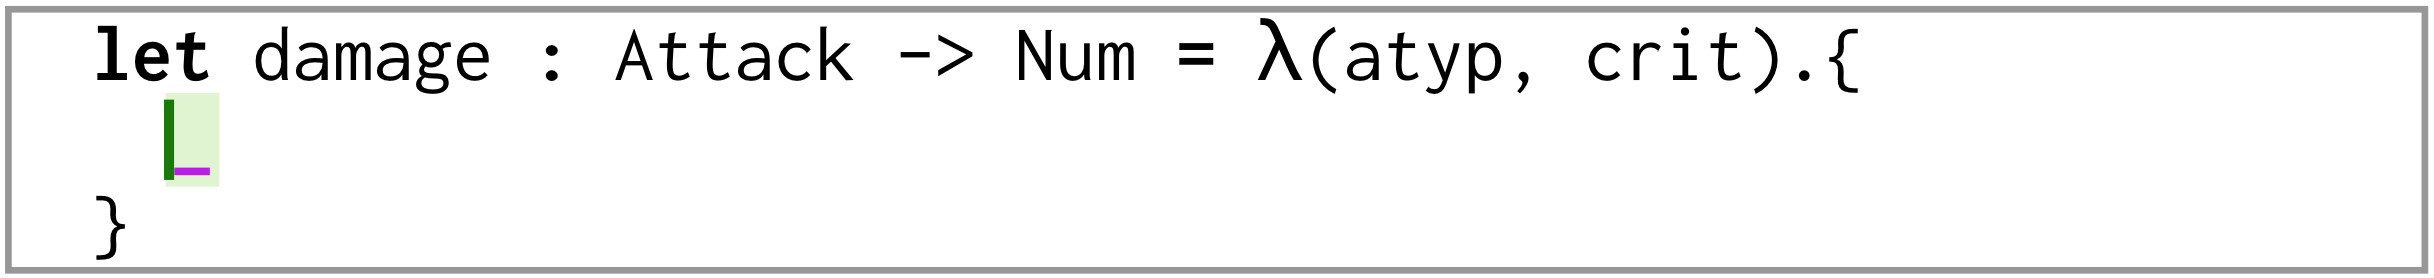
\includegraphics[width=\linewidth]{fig/context.png}\par
}
\noindent
All following listings should be interpreted as filling the body of the \texttt{damage} function.

{\centering
	\vspace{-0.1cm}
  $\vdots$\par
  \vspace{0.1cm}
}
\noindent
Suppose we have so far implemented \texttt{damage} as follows.

{\centering
  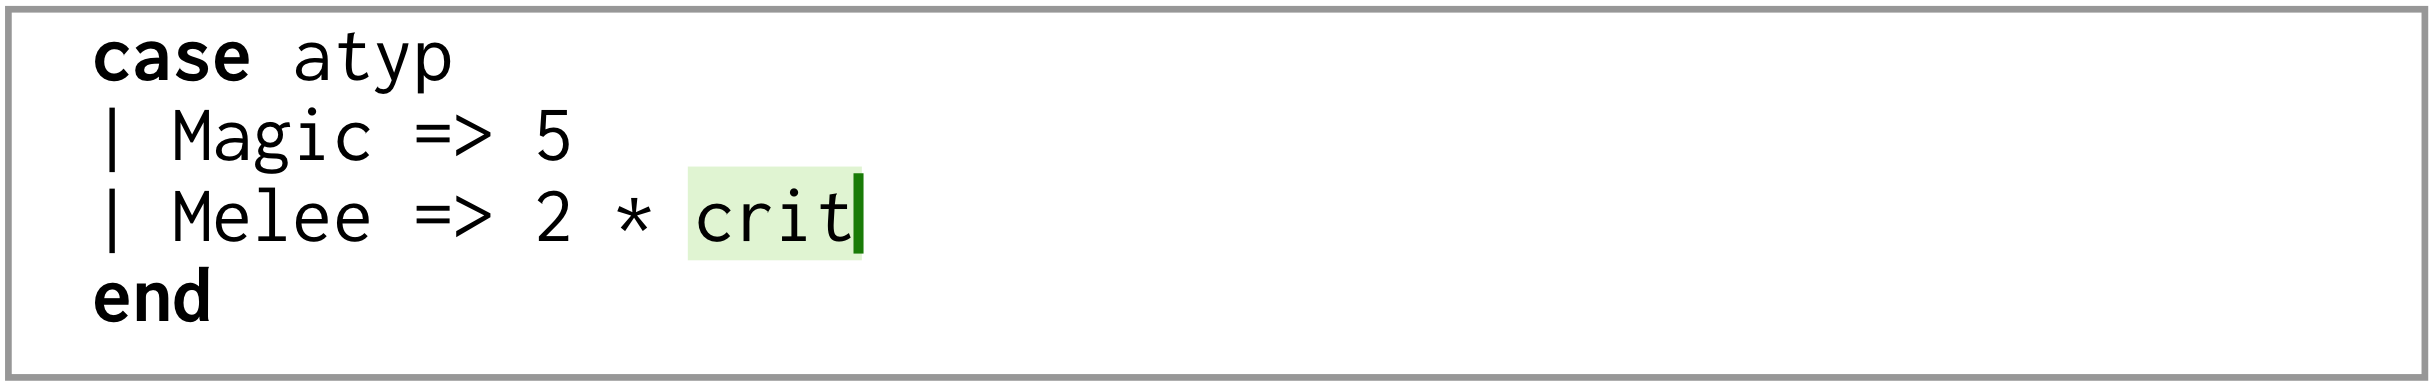
\includegraphics[width=\linewidth]{fig/frame1.png}\par
}
\noindent
%\begin{tabular}{|p{\linewidth}}
We press keys \key{+} and \key{1}.
%\end{tabular}

{\centering
  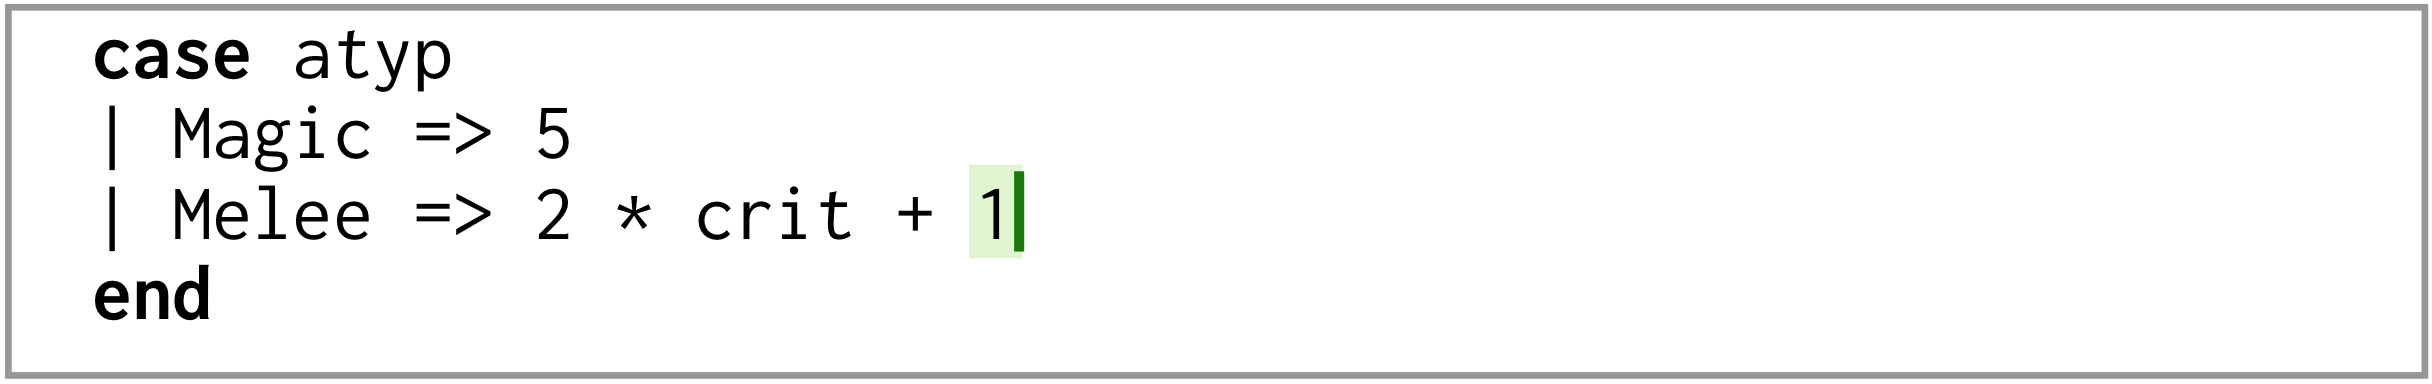
\includegraphics[width=\linewidth]{fig/frame2.png}\par
}
\noindent
A naïve structure editor design would maintain a strict tree structure and apply
	edit commands as context-free transformations. \Hazel avoids this issue via
	Feature \feat{2}, while \Hazel's edit actions re-parse operator precedence as
	needed for typchecking. This approach is similar to MPS's side transformations \cite{GrammarCells}.

{\centering
	\vspace{-0.1cm}
  $\vdots$\par
  \vspace{0.1cm}
}
\noindent
We have in scope the player's \texttt{defenseScore}
	and want to integrate it into the damage calculation.
Our plan is to bind the current expression to a new variable \texttt{attackScore}
	and return a damage score in terms of \texttt{attackScore} and \texttt{defenseScore}.

{\centering
  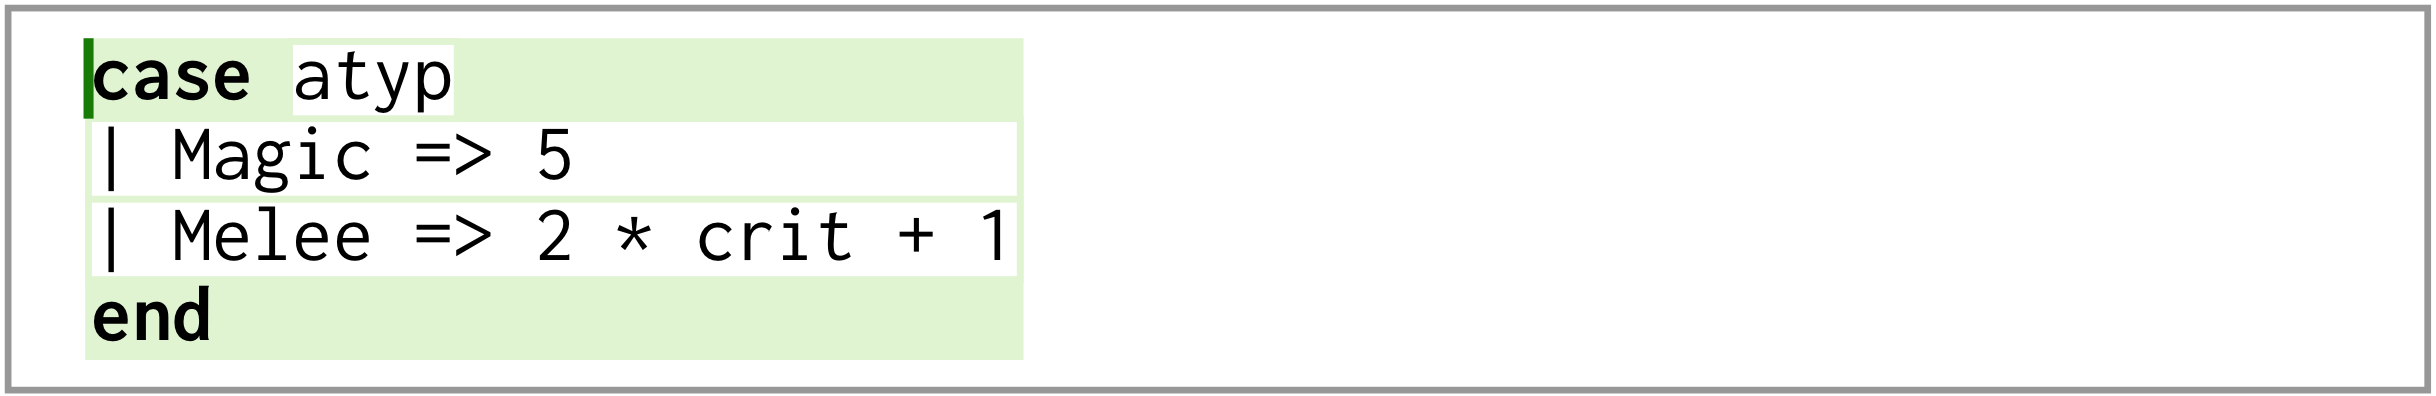
\includegraphics[width=\linewidth]{fig/frame3.png}\par
}
\noindent
%\begin{tabular}{|p{\linewidth}}
We have moved the cursor to the start of the \texttt{case} expression.
Note that the dark green caret is augmented with a light green shading of the
	the \texttt{case} node and outlines of its child nodes [Feature \feat{3}].
	
We press \key{Enter} to create a new empty line.
Direct encoding of line items allows us to create space around existing nodes
	in preparation for a complex node construction, just like in a text editor.
%\end{tabular}

{\centering
  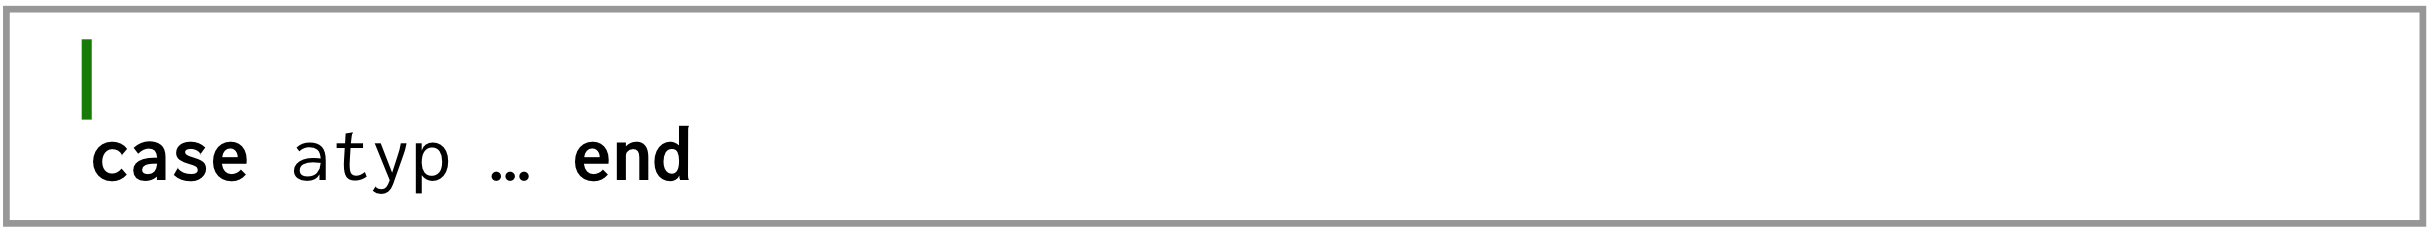
\includegraphics[width=\linewidth]{fig/frame4.png}\par
}
\noindent
%\begin{tabular}{|p{\linewidth}}
We type the keys \key{l} \key{e} \key{t} \key{Space} to construct a new let line.
%\end{tabular}

{\centering
  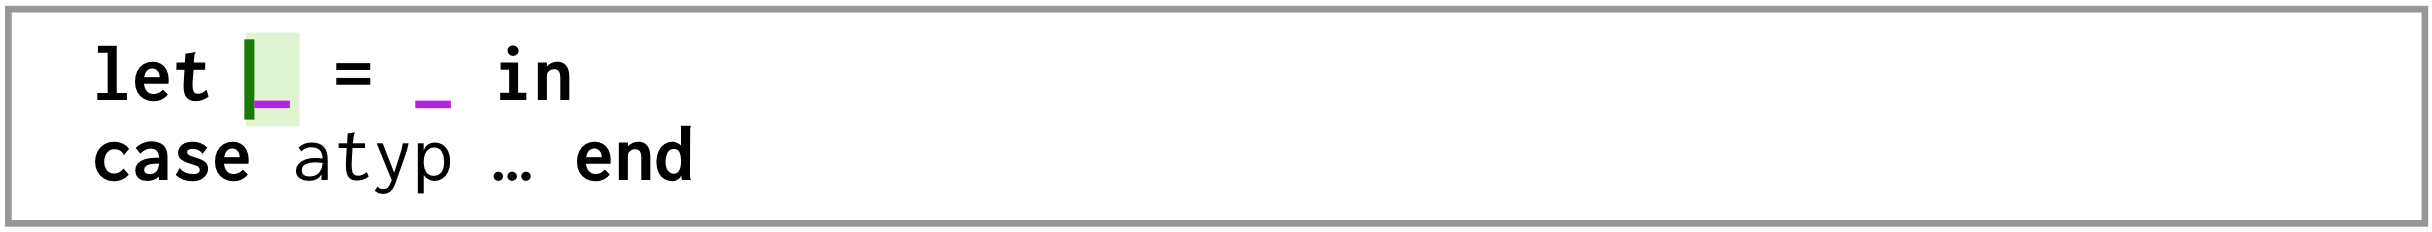
\includegraphics[width=\linewidth]{fig/frame5.png}\par
}
\noindent
By recognizing keywords that prefix syntactic forms, \Hazel eliminates the requirement
	to learn keyboard shortcuts.

{\centering
	\vspace{-0.1cm}
  $\vdots$\par
  \vspace{0.1cm}
}
\noindent

{\centering
  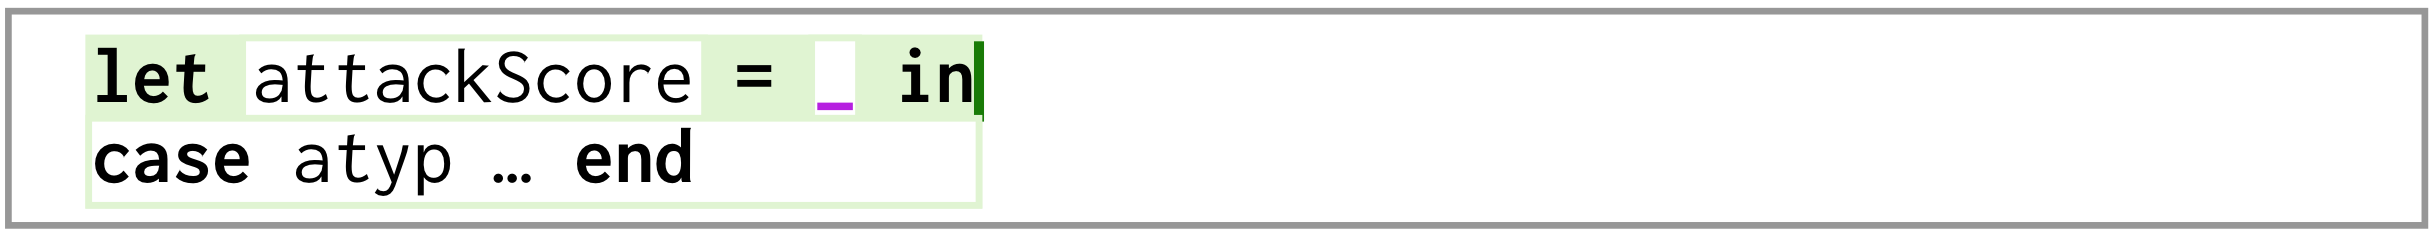
\includegraphics[width=\linewidth]{fig/frame6.png}\par
}
\noindent
Now that we have created \texttt{attackScore}, we want to bind it
	to the \texttt{case} expression on the following line.
In a text editor, we would delete the delimiter \texttt{in} and retype it after
	the \texttt{case} expression. Similarly, we hit \key{Backspace}.

{\centering
  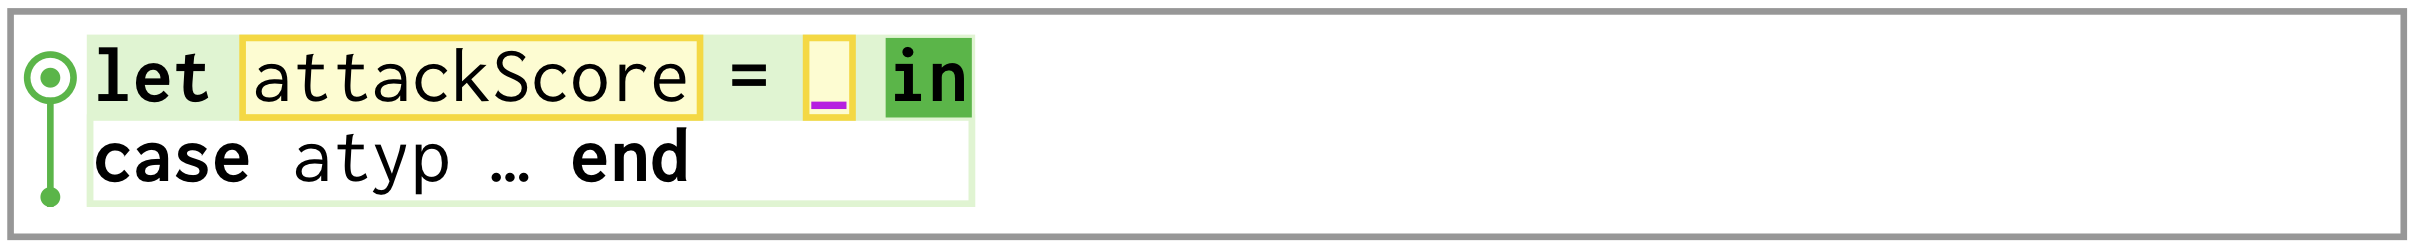
\includegraphics[width=\linewidth]{fig/frame7.png}\par
}
\noindent
We have entered \emph{node staging mode} [Feature \feat{4}].
Just as a code completion menu facilitates exploration of valid token completions,
	node staging mode facilitates exploration of valid placements of a node's
	syntactic delimiters.
The \texttt{in} delimiter is highlighted in dark green to indicate that it is
	the delimiter to be placed, while the dark green guide on the left signifies
	possible positions.
The two children nodes of the let line are highlighted to indicate that, if
	we were press \key{Backspace} again, they would be deleted as well.

We press \key{$\rightarrow$} or \key{$\downarrow$} to move \texttt{in} to the next position.

{\centering
  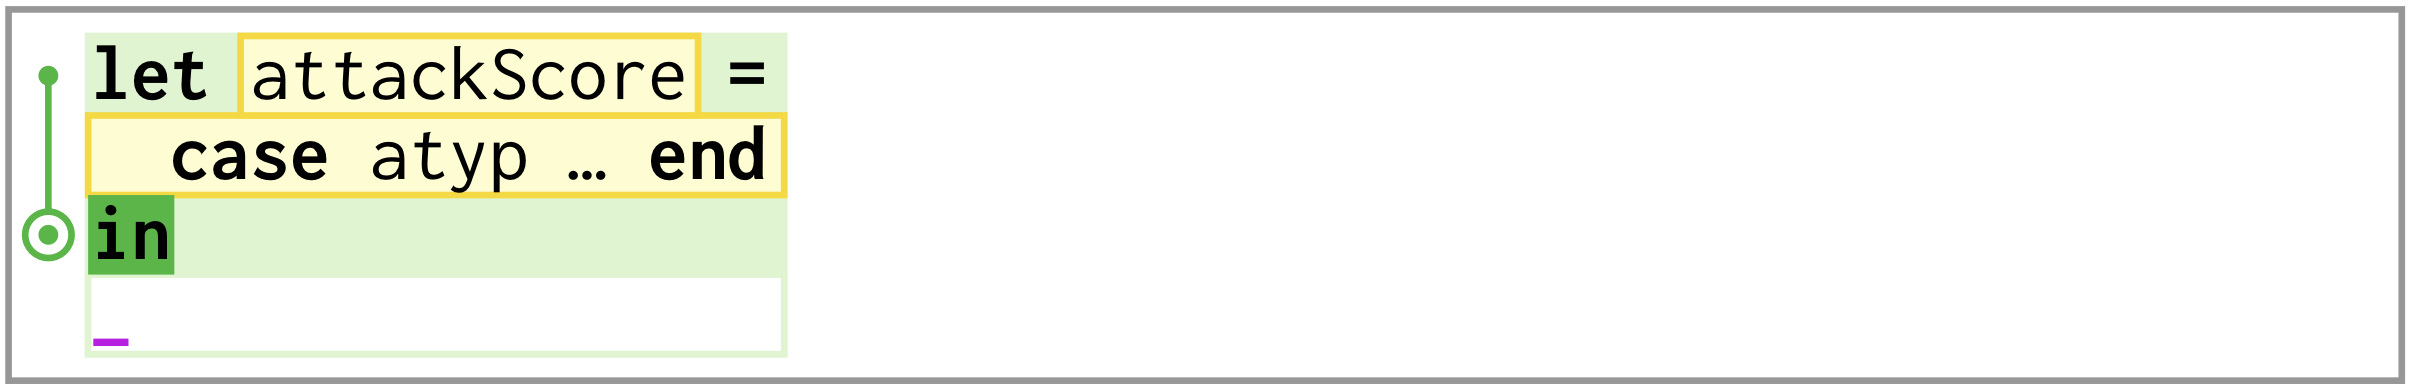
\includegraphics[width=\linewidth]{fig/frame8.png}\par
}
\noindent
We press \key{Enter} to accept this position and return to normal editing mode.

{\centering
  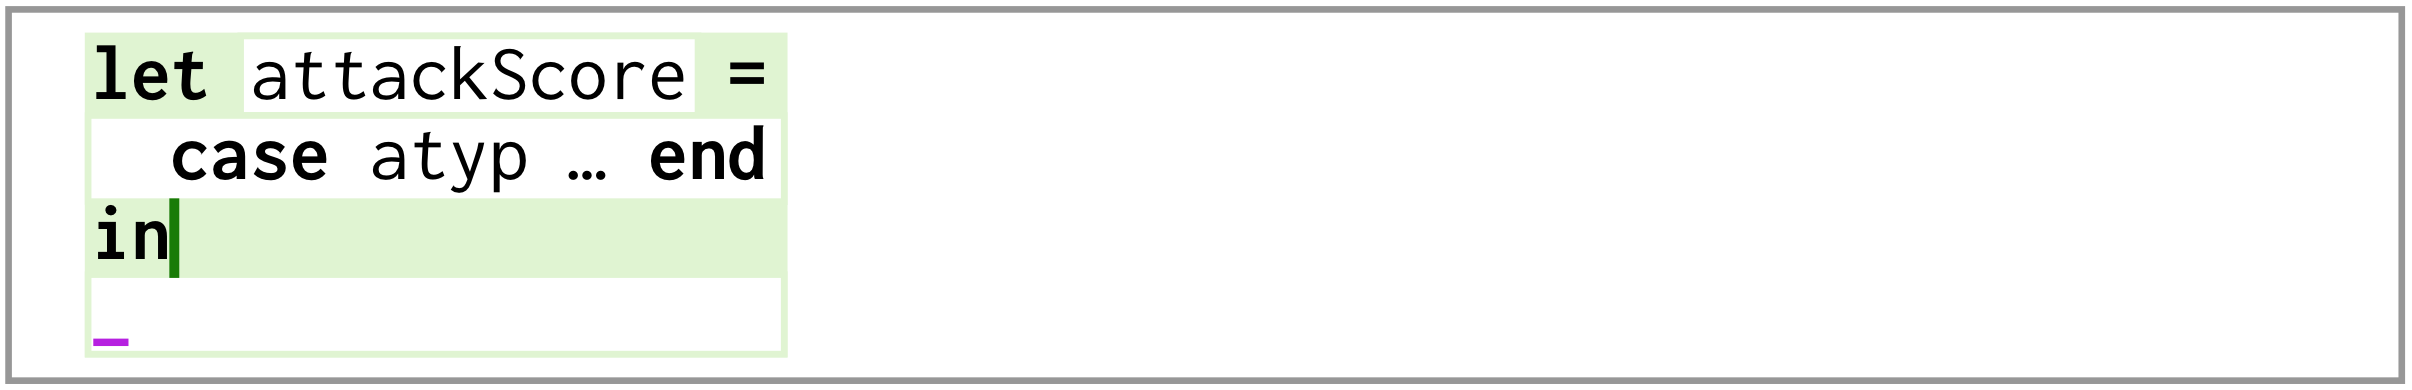
\includegraphics[width=\linewidth]{fig/frame9.png}\par
}
\noindent
Note the similarity in keystrokes to the text editor experience.

{\centering
	\vspace{-0.1cm}
  $\vdots$\par
  \vspace{0.1cm}
}
\noindent

{\centering
  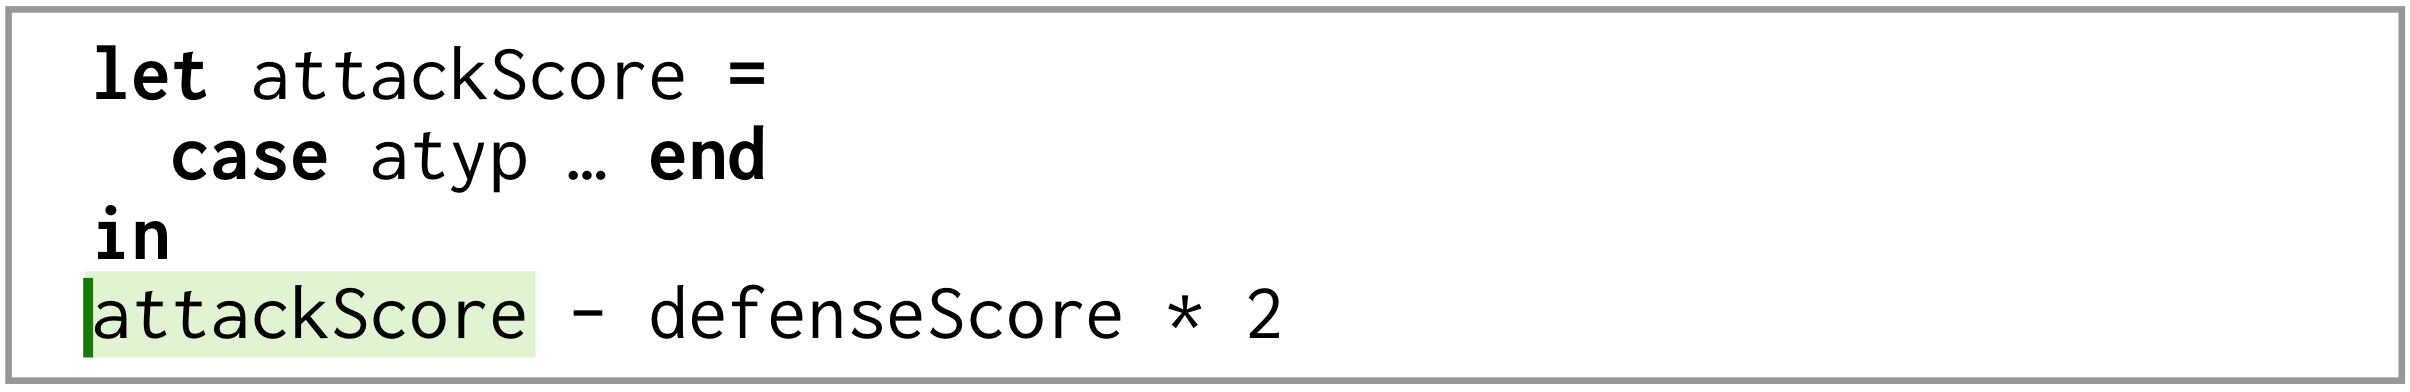
\includegraphics[width=\linewidth]{fig/frame10.png}\par
}
\noindent
We have entered our final calculation but have forgotten to account for operator precedence.
We press \key{(} at the start of the return expression.

{\centering
  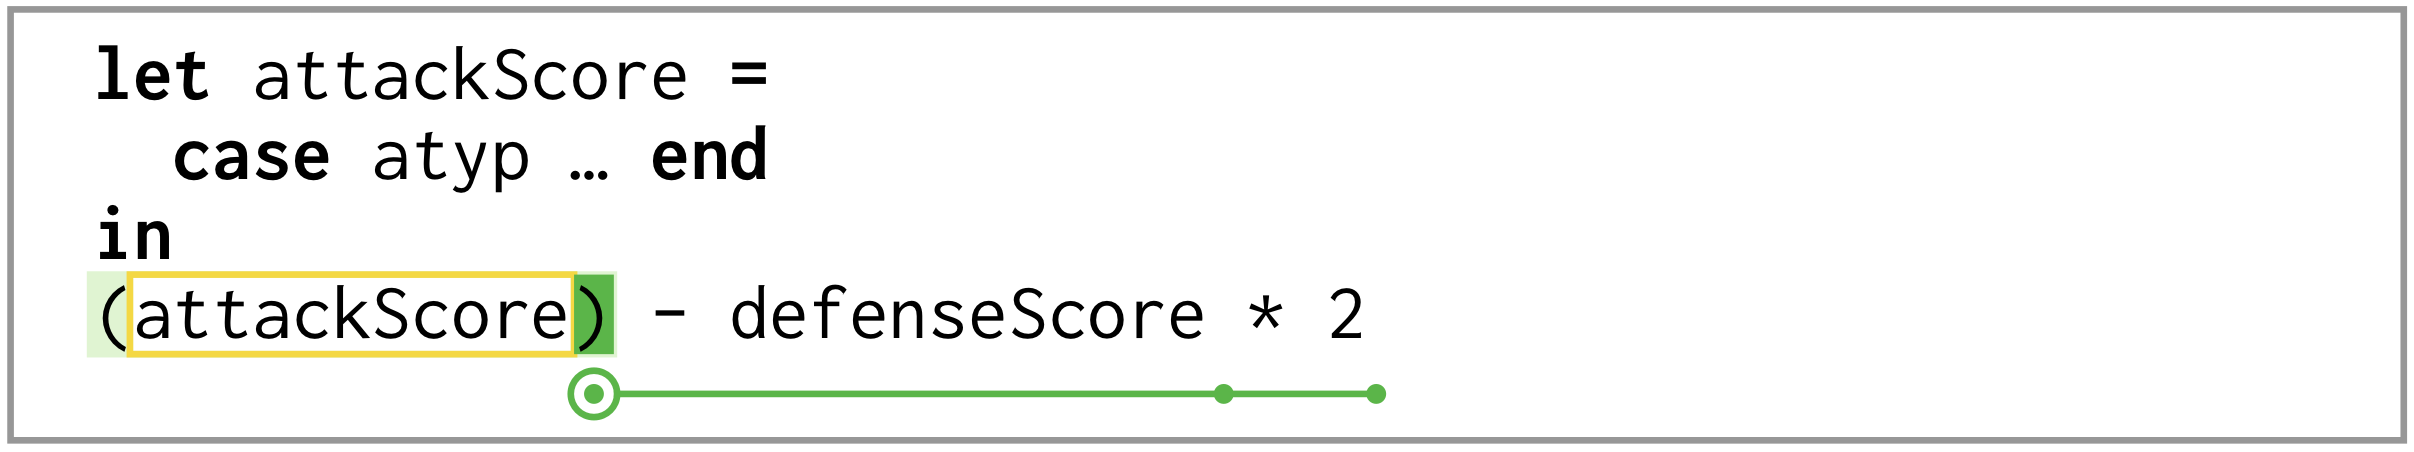
\includegraphics[width=\linewidth]{fig/frame11.png}\par
}
\noindent
In the case of parentheses, \Hazel enters node staging mode automatically if it detects
	ambiguity in intent.
We press \key{$\rightarrow$} for the next position.

{\centering
  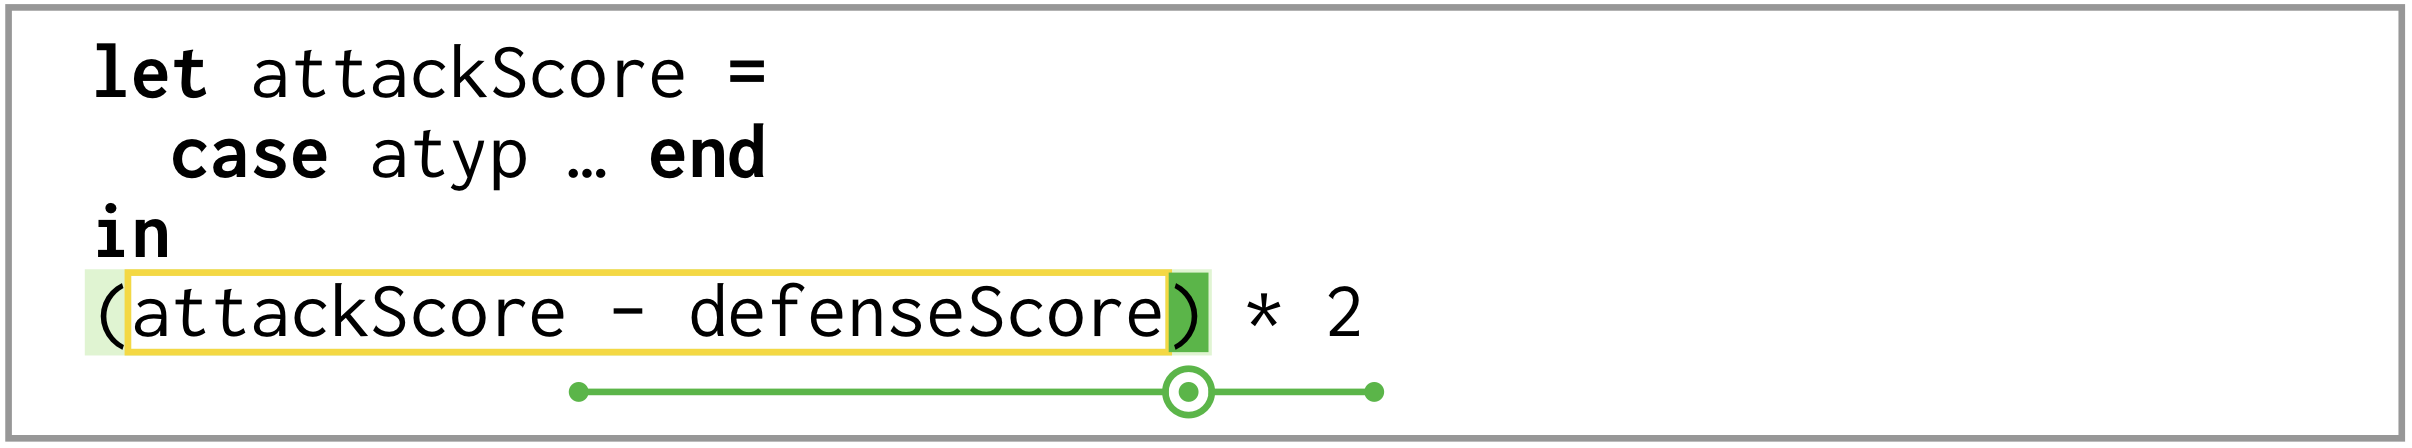
\includegraphics[width=\linewidth]{fig/frame12.png}\par
}
\noindent
Finally we press \key{Enter} or \key{)} to accept and exit node staging. 

{\centering
  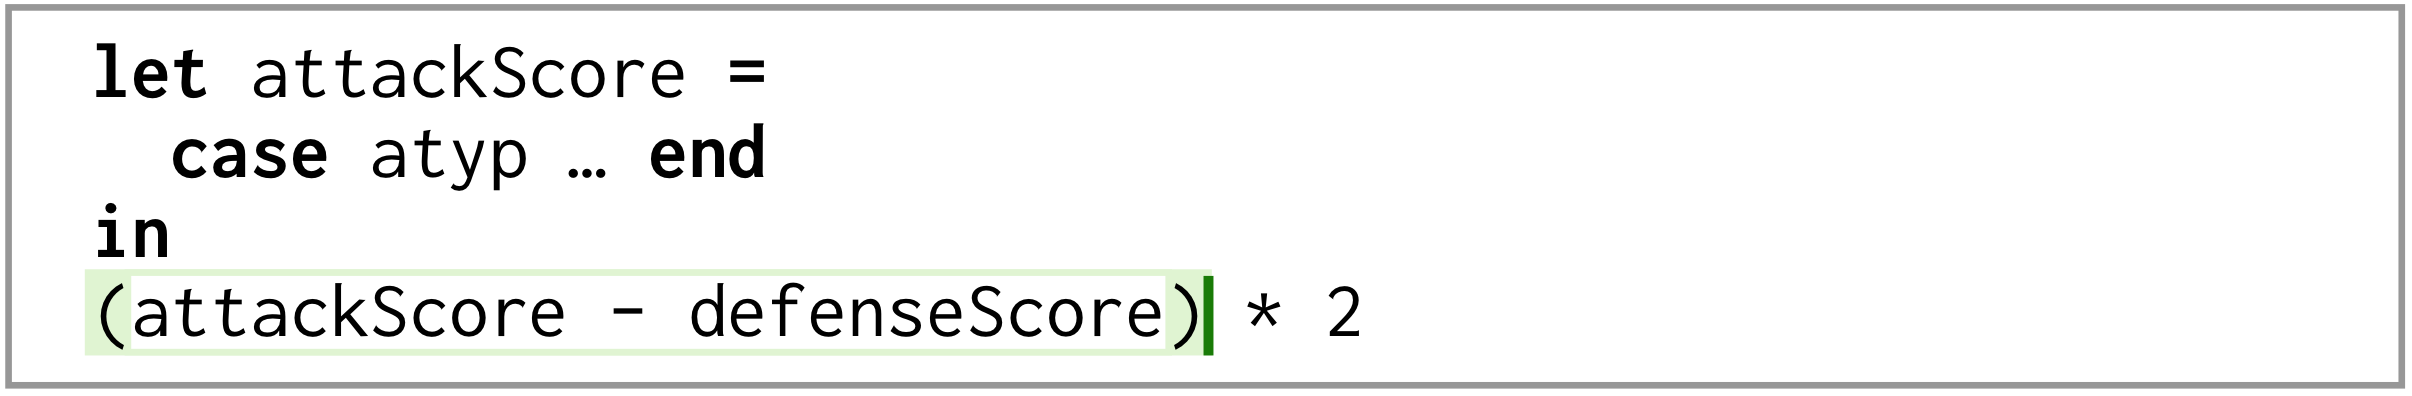
\includegraphics[width=\linewidth]{fig/frame13.png}\par
}
\noindent
Once again,
note the similarity in keystrokes to the text editor experience.

\newpage
\bibliography{refs}

\end{document}